\documentclass[12pt]{article}
\usepackage{graphicx}
\usepackage[utf8]{inputenc}
\usepackage[spanish,mexico]{babel}
\usepackage{float}
\usepackage{hyperref}


\begin{document}


\newpage

\thispagestyle{empty}
\begin{center}

 
  {\Huge \bf Anteproyecto}

  \vspace*{2cm}
  {\LARGE\bf Programaci\'on de Dispositivos M\'oviles}
  
  \vspace*{0.45cm}
  
  \vfill

  {\large Emerson Gamaliel Nolasco Cornejo 00215316\\
           Karla Lissette Cruz Mendoza 00010216\\
   Kevin Enmanuel Vel\'asquez Mendoza 00018616\\
           Kevin Alexander L\'opez Aquino 00251716\\
            [3mm] \textbf{Catedr\'atico:} Lic. N\'estor Aldana}
  \vspace*{0.9cm}
  

   \begin{center}
   
\includegraphics[scale=0.7]{img/uca.png}
   \end{center}
	\vspace*{10mm}
  {\large Departamento de Electr\'onica e Inform\'atica\\
   Universidad Centroamericana "Jos\'e Sime\'on Ca\~nas"\\
           El Salvador\\
          [1mm]  Marzo de 2018}

\end{center}

\newpage
\setcounter{page}{2}
\fontsize{15}{18}\selectfont

\section{Objetivos y resultados esperados} 

El objetivo principal es proveer a la comunidad estudiantil una aplicación que facilite el intercambio de información y además esté bien diseñada, funcione de manera eficiente y sea fácil de usar. Teniendo en cuenta esto, se esperaría presentar el resultado final a estudiantes y personal de la universidad para considerar su implementación.

\begin{figure}[H]
	\caption{\textbf{Login de usuario}}
	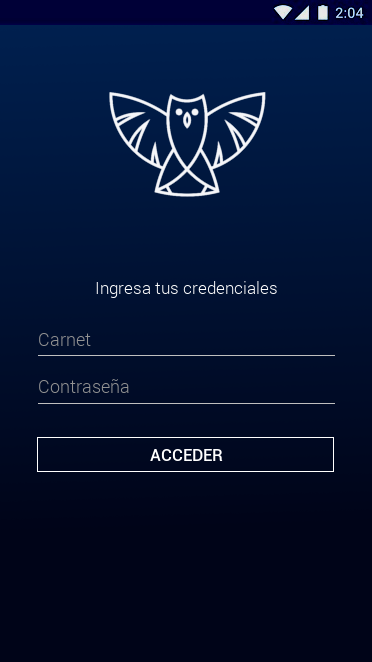
\includegraphics[scale=0.50]{img/1.png}
	\centering
\end{figure}

\section{Metodología} 


La primera parte del diseño será analizar la estructura de la universidad y las relaciones entre los diferentes entes que comparten información y el tipo de información para poder modelar esto en una base de datos a forma de demo, con registros producidos al azar para las pruebas iniciales. A partir de esto, comenzaríamos a construir las partes señaladas en la descripción del proyecto. Todos los participantes estarán involucrados en el proyecto de desarrollo, trabajando por metas: al cumplir con una se asigna otra y de esa manera hasta que se ha finalizado el proyecto.

\begin{figure}[H]
	\caption{\textbf{Men\'u}}
	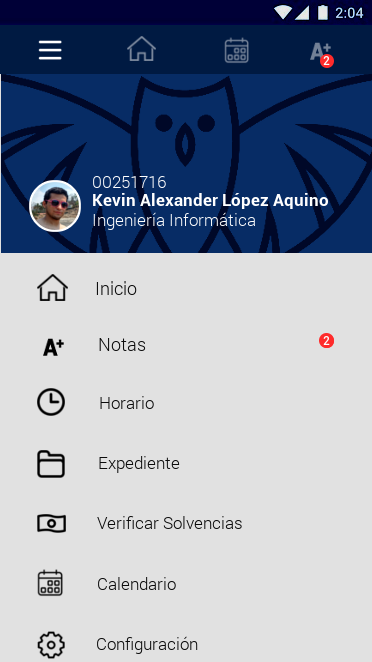
\includegraphics[scale=0.45]{img/5.png}
	\centering
\end{figure}


\section{Descripción general del proyecto}

Cuando se trata de intercambiar información con sus estudiantes, la universidad debe tener en cuenta las aplicaciones móviles porque virtualmente la gran mayor\'ia tienen un dispositivo con el cual pueden recibir información y solicitarla de forma más rápida que a través de otros medios. Si bien esto se logra parcialmente con el correo electrónico y las aplicaciones web dedicadas a este, una aplicación m\'ovil especializada para información universitaria permitiría realizar esta transmisi\'on de informaci\'on de manera más directa: se podrían atender varias necesidades de los estudiantes en un solo lugar, a través de una sola aplicación y se podría intercambiar más contenido.
\newline El proyecto consiste en desarrollar una aplicación que tenga las siguientes funcionalidades: 
\newline
\newline
\textbf{a. Horarios diarios} donde el estudiante puede consultar qué actividades académicas tiene en un día específico y el lugar donde se realizarán. Véase la Figura~\ref{fig:horarioDiario}.
\newline
\newline
\textbf{b. \textit{News feed}} que puede estar al iniciar la aplicación y donde se puede colocar la cartelera estudiantil semanal, avisos sobre pagos, invitaciones a eventos, entre otra información que usualmente se recibe por correo electrónico. Véase la Figura~\ref{fig:newsFeed}.  
\newline
\newline
\textbf{c. Sistema de consulta de notas y estadísticas académicas } que brindarían acceso a información como la que provee el expediente personal en el Portal de Estudiantes pero de forma mucho más rápida, disponible en el bolsillo en cualquier momento. Véase la Figura~\ref{fig:consultaNotas}.

\begin{figure}[H]
	\caption{\textbf{Horario diario}}
	\label{fig:horarioDiario}
	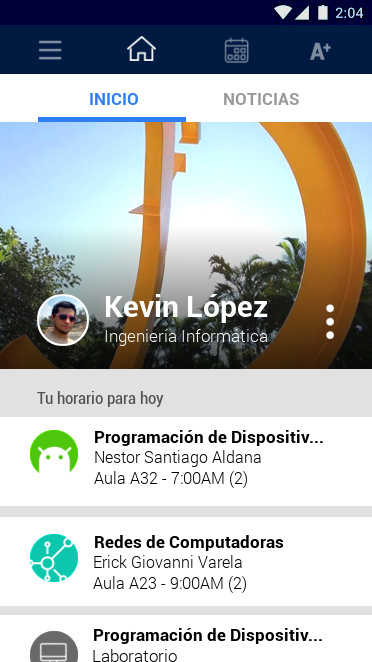
\includegraphics[scale=0.50]{img/2.png}
	\centering
\end{figure}

\setlength{\parindent}{0cm}
\textbf{d. Calendario académico} para ser visualizado en cualquier momento y añadir eventos además de los que la universidad tenga previstos en su calendario oficial. Estos eventos pueden ser, por ejemplo, discusiones, laboratorios, entregas de proyectos. Véase la Figura~\ref{fig:calendario}.
\newline
\newline
\textbf{e. Verificar estado de solvencia. } Capacidad para llevar un control de los pagos ya realizados y pr\'oximos a realizar (indicando su respectiva fecha de ejecuci\'on, monto y fecha de vencimiento). 

\begin{figure}[H]
	\caption{\textbf{News feed}}
	\label{fig:newsFeed}
	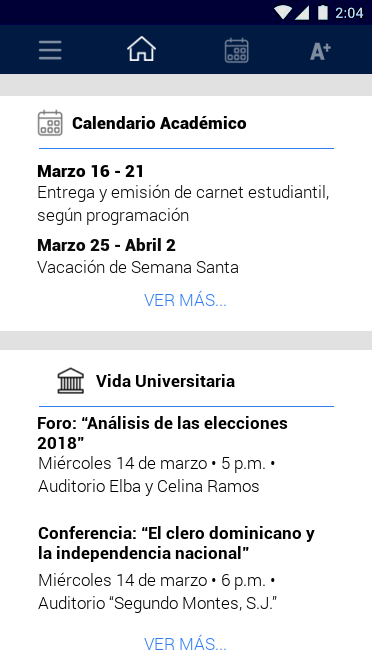
\includegraphics[scale=0.50]{img/3.png}
	\centering
\end{figure}


\textbf{f. Notificaciones inteligentes. }Recordatorios determinados seg\'un  datos de inter\'es al estudiante, por ejemplo: evaluaciones pr\'oximas, calendario UCA, eventos relacionados con su \'area, expiraciones en las fechas de pago de mensualidad, entregas de libros pendientes en biblioteca.\\

\begin{figure}[H]
	\caption{\textbf{Consulta de notas}}
	\label{fig:consultaNotas}
	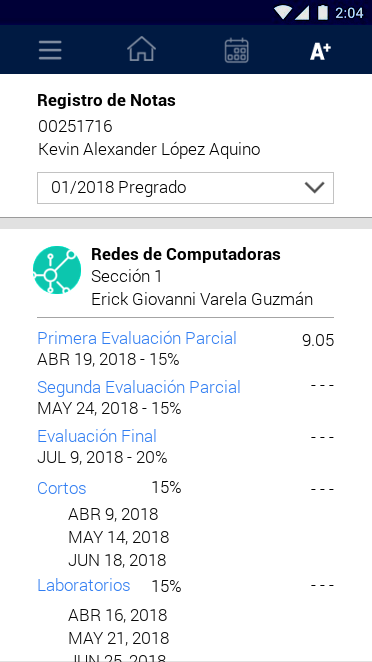
\includegraphics[scale=0.50]{img/6.png}
	\centering
\end{figure}

\begin{figure}[H]
	\caption{\textbf{Calendario}}
	\label{fig:calendario}
	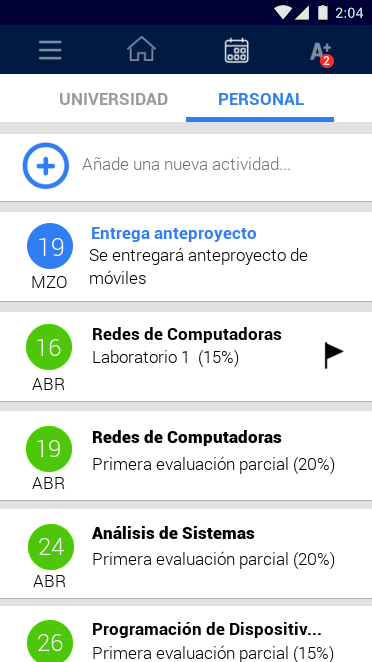
\includegraphics[scale=0.50]{img/4.png}
	\centering
\end{figure}


\end{document}